\documentclass{beamer}

\usepackage[utf8]{inputenc}
\usepackage[T1]{fontenc}
\usepackage{amsmath}
\usepackage{bm}

\usepackage{tabularx}
\usepackage{graphicx}
\usepackage{epstopdf}

\graphicspath{{../../images/}}

\usetheme{Madrid}
\usebeamercolor{sidebartab}
\usefonttheme{professionalfonts}


\title[M.Sc. Thesis 2015]{Spatial Summarization of Image Collections}
\author{Diego A. Ballesteros Villamizar}
\institute[ETHZ]{ETH Zürich}
\date{December 14th, 2015}

\DeclareMathOperator*{\argmin}{argmin}
\DeclareMathOperator*{\argmax}{argmax}

\AtBeginSection[]
{
  \begin{frame}<beamer>
    \frametitle{Outline}
    \tableofcontents[currentsection]
  \end{frame}
}

\begin{document}

  \begin{frame}
    \titlepage
  \end{frame}
  
  \section{Bug squashing}
  
  \begin{frame}{Fixed baseline models}
    \begin{itemize}
      \item Proximity model had a very low accuracy in last report.
      \item Code generating the list of items was mixing up the indexes.
      \item After fixing that bug, the proximity model improved its results.
      \item Markov model without rejection of items in the set was also applied
    \end{itemize}
  \end{frame}
  
  \begin{frame}{Ranking test generation}
    \begin{itemize}
      \item For every set in the test data, the ranking test is generated from all combinations taking out an item.
      \item Order of the original sets is not preserved.
      \item This should be considered in the Markov and Proximity models.
      \item For Markov, the sum of the transition probabilities is used for generating the recommended items.
      \item For the Proximity model, the mininum distance from any item in the partial set is used for ranking.
    \end{itemize}
  \end{frame}
  
  \begin{frame}{Fixed results}
    \begin{table}
      \begin{tabularx}{0.7\textwidth}{X|c|c|c|c}
        Model         & $Acc$ & $\sigma_{Acc}$ & $MRR$ & $\sigma_{MRR}$ \\
        \hline
        Modular       & 18.15 & 3.08           & 45.80 & 1.73 \\
        Proximity     & 26.38 & 2.78           & 47.19 & 1.92 \\
        FLID ($d=10$) & 28.34 & 4.07           & 51.76 & 2.52 \\
        Markov        & 32.07 & 2.69           & 52.40 & 1.76 \\
        Proximity with rejection     & 34.60 & 3.29           & 55.88 & 2.15 \\
        Markov with rejection & 36.50 & 3.10           & 57.91 & 1.89
      \end{tabularx}
    \end{table}
  \end{frame}
  
  \begin{frame}{Diversity Encoding ($d=10$)}
    \begin{figure}
      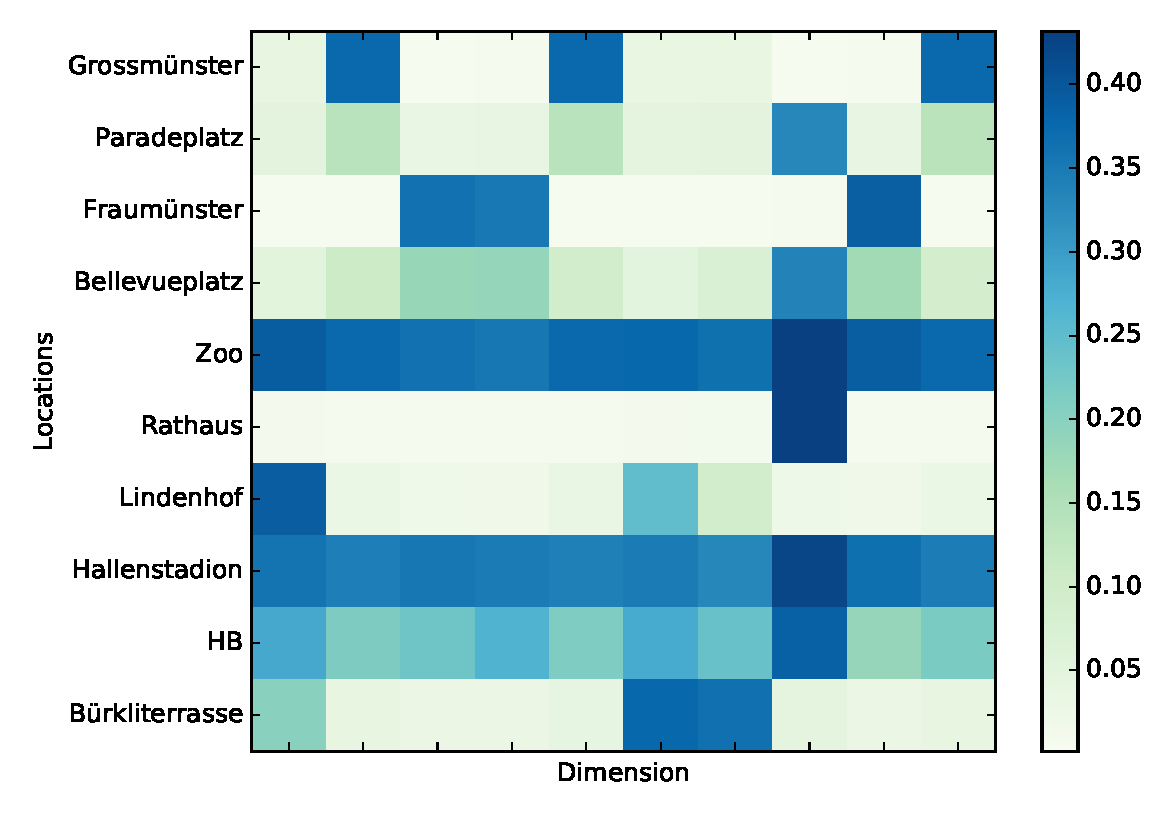
\includegraphics[width=0.7\textwidth]{submodular_weights_d_10}
    \end{figure}
  \end{frame}
  
  \section{Featurization}
  
  \begin{frame}{Sanity test}
    \begin{itemize}
      \item Setting $\bm{X} = \mathbb{I}$ simplifies the featurized model to the original FLID model.
      \item $M = \lvert \bm{V} \rvert$
      \item $\bm{W} = \bm{X}\bm{B} = \bm{B}$
      \item $\bm{u} = \bm{X}\bm{a} = \bm{a}$
    \end{itemize}
    \begin{table}
      \begin{tabularx}{0.7\textwidth}{X|c|c|c|c}
        Model         & $Acc$ & $\sigma_{Acc}$ & $MRR$ & $\sigma_{MRR}$ \\
        \hline
        FFLID ($d=2$)  & 20.88 & 2.28           & 47.15 & 1.48 \\
        FFLID ($d=5$)  & 27.09 & 4.30           & 50.69 & 2.65 \\
        FFLID ($d=10$) & 28.34 & 4.07           & 51.76 & 2.52
      \end{tabularx}
    \end{table}
  \end{frame}
  
  \begin{frame}{Automatic features}
    \begin{itemize}
      \item From the Flickr data: Latitude, longitude, number of photos, number of users.
      \item Scaled to $[0,1]$.
      \item $m = 4$.
    \end{itemize}
    \begin{table}
      \begin{tabularx}{0.7\textwidth}{X|c|c|c|c}
        Model          & $Acc$ & $\sigma_{Acc}$ & $MRR$ & $\sigma_{MRR}$ \\
        \hline
        FFLID ($d=2$)  & 18.75 & 3.19 & 45.97 & 1.84 \\
        FFLID ($d=5$)  & 18.98 & 3.18 & 46.08 & 1.85 \\
        FFLID ($d=10$) & 19.02 & 3.21 & 46.16 & 1.84
      \end{tabularx}
    \end{table}
  \end{frame}
  
    \begin{frame}{Diversity Encoding ($d=10$)}
      \begin{figure}
        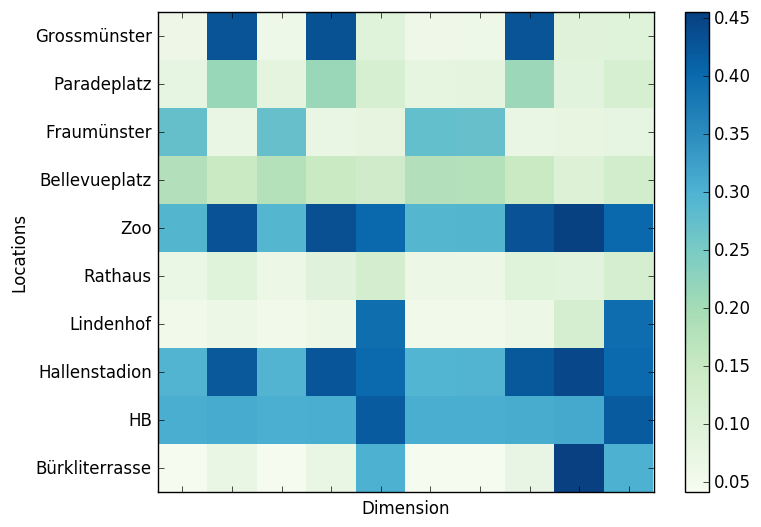
\includegraphics[width=0.7\textwidth]{submodular_weights_f_1_d_10}
      \end{figure}
    \end{frame}
  
  \begin{frame}{Augmented features}
    \begin{itemize}
      \item Previous features, augmented with the identity matrix.
    \end{itemize}
    \begin{table}
      \begin{tabularx}{0.7\textwidth}{X|c|c|c|c}
        Model          & $Acc$ & $\sigma_{Acc}$ & $MRR$ & $\sigma_{MRR}$ \\
        \hline
        FFLID ($d=2$)  & 19.21 & 2.97 & 46.21 & 1.83 \\
        FFLID ($d=5$)  & 22.20 & 4.29 & 47.99 & 2.52 \\
        FFLID ($d=10$) & 25.66 & 4.08 & 50.00 & 2.73
      \end{tabularx}
    \end{table}
  \end{frame}
  
  \begin{frame}{Diversity Encoding ($d=10$)}
    \begin{figure}
      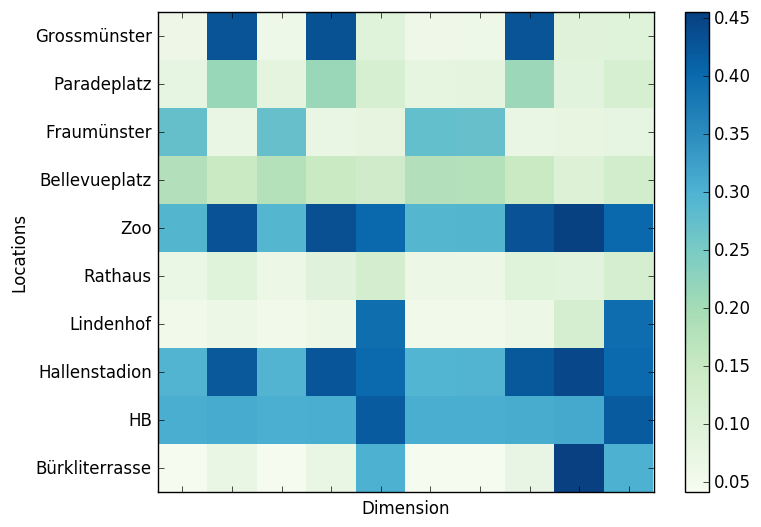
\includegraphics[width=0.7\textwidth]{submodular_weights_f_2_d_10}
    \end{figure}
  \end{frame}
  
  
  
  \section{Conclusion}
  
  \begin{frame}{Observations}
    \begin{itemize}
      \item FLID with 10 dimensions can encode the different combinations in the data.
      \item FFLID tries to the learn the same $\bm{W}$ but if the number of parameters is smaller, the score is worse.
      \item Markov and Proximity models are simple but perform the best.
      \item Binary features end up encoding each item. All items have different characteristics, except the churches.
      \item Diversity may not be the best model of the tourist behavior, e.g. people go to both churches.
    \end{itemize}
  \end{frame}
  
  \begin{frame}{Next steps}
    \begin{itemize}
      \item Choosing more items could help FFLID as there is more variation in the features.
      \item Adding coherence should produce better results.
    \end{itemize}
  \end{frame}

\end{document}
